% Template for Elsevier CRC journal article (Procedia Computer Science)
% Filled in from the base template for: VideoRAG for Courtroom Evidence
%
% NOTE ON COMPILATION: this file uses the exact frontmatter conventions of
% the Procedia template you supplied (\usepackage{ecrc}, \jid, \dochead,
% etc.). ecrc.sty is distributed directly inside Elsevier's Procedia author
% kit (the same place this .tex template came from) rather than through
% public LaTeX package archives, so it was not available to compile-check
% in the sandbox this was written in. The document was hand-verified for
% balanced environments/braces and otherwise follows elsarticle's standard
% conventions throughout; compile with your existing template kit or on
% Overleaf (search "Elsevier - Procedia") for a fast first build.

\documentclass[3p,times,procedia]{elsarticle}
\flushbottom

\usepackage{ecrc}
\usepackage{graphicx}
\usepackage[bookmarks=false]{hyperref}
    \hypersetup{colorlinks,
      linkcolor=blue,
      citecolor=blue,
      urlcolor=blue}
\usepackage{amsmath}
\usepackage{booktabs}
\usepackage{subcaption}

\volume{00}
\firstpage{1}
\journalname{Procedia Computer Science}
\runauth{Kavinesh et al.}
\jid{procs}

\usepackage[figuresright]{rotating}

\begin{document}
\begin{frontmatter}

\dochead{International Conference on Machine Learning and Data Engineering}

\title{VideoRAG for Courtroom Evidence: Cross-Session Speaker Identification, Testimony Contradiction Detection, and Citation-Verified Video Question Answering}

\author[a]{Kavinesh P}
\author[a]{Raam Prathap R V}
\author[a]{Santhosh A S}
\author[a]{Kasam Sai Venkata Siddardha}
\author[a]{Ashish M}
\author[a]{M Anbazhagan\corref{cor1}}

\address[a]{Department of Computer Science and Engineering, Amrita School of Computing, Coimbatore 641112, Amrita Vishwa Vidyapeetham, India}

\begin{abstract}
Reviewing hours of recorded courtroom testimony for inconsistencies, and locating the
exact moment a claim was made, is a slow, manual process for legal teams. We present a
multimodal Retrieval-Augmented Generation (RAG) system for courtroom video evidence
that decomposes a natural-language query into structured retrieval requests across
speech transcription, on-screen text, object detection, and visual-similarity indexes,
then merges the retrieved evidence into a single grounded answer. Beyond this base
architecture we contribute three layers aimed specifically at legal use: (1)
cross-session speaker identification, which matches a witness's voice across separately
uploaded recordings using cosine similarity over speaker embeddings, gated by a
human-confirmation step before any match is trusted downstream; (2) persistent
testimony memory, which stores every attributable statement a speaker makes across
sessions and flags factual contradictions with an LLM classifier, timestamps, and
explanations; and (3) citation verification, which independently checks that every
timestamp cited in a generated answer actually supports its claim, and computes a
SHA-256 hash of the cited clip for tamper evidence. We evaluate all layers with seven
targeted experiments against a corpus that includes real public-domain speech
recordings and real courtroom trial footage, reporting standard metrics (Recall@k,
MRR, ROC-AUC, EER, precision/recall/F1) alongside two honestly-reported negative
findings — weak caption/OCR retrieval, and an image-search confidence threshold
miscalibrated for real-world class imbalance — each with a concrete, data-backed
remediation recommendation.
\end{abstract}

\begin{keyword}
video retrieval-augmented generation \sep legal video analysis \sep speaker diarization \sep testimony contradiction detection \sep citation verification \sep multimodal question answering
\end{keyword}
\cortext[cor1]{Corresponding author: M Anbazhagan}
\end{frontmatter}

\email{m\_anbazhagan@cb.amrita.edu}

\vspace*{-6pt}

\section{Introduction}
\label{sec:intro}

Courtroom proceedings are increasingly recorded and, in many jurisdictions, livestreamed,
producing large volumes of video evidence that legal teams must review by hand. Two
tasks in particular are labor-intensive: locating the specific moment a witness said
something relevant to a case, in a recording that may run for hours, and checking
whether a witness's account is internally consistent, both within one session and
across every session they have testified in, which may span days or weeks of
proceedings. General-purpose video question-answering systems address the first
problem for a single clip; they have no mechanism for recognizing the same speaker
across separate uploads, no memory of what a person has said in earlier sessions, and
no step that verifies a generated answer's citations are actually supported by the
underlying footage before presenting them as fact.

This paper describes a system built to close those three gaps directly. Its
contributions are:
\begin{itemize}
\item A base multimodal RAG architecture that decomposes a query into a structured
retrieval request (Query Decouple), routes it across automatic speech recognition
(ASR), optical character recognition (OCR), object detection, and CLIP-based visual
similarity indexes, and merges the results into one grounded answer (Section
\ref{sec:arch}).
\item \textbf{Cross-session speaker identification}: voiceprint extraction and
cosine-similarity matching against a per-case speaker registry, with every automatic
match held for human confirmation before it is trusted by the contradiction-detection
layer below (Section \ref{sec:novelty1}).
\item \textbf{Persistent testimony memory and contradiction detection}: every
attributable statement is stored against a canonical speaker identity across sessions,
and new statements are checked against that speaker's prior statements with an LLM
classifier that reports a label, confidence, and explanation (Section
\ref{sec:novelty2}).
\item \textbf{Citation verification}: a second, independent check that a generated
answer's cited timestamps genuinely support its claims, with a SHA-256 hash of the
cited clip for tamper evidence (Section \ref{sec:novelty3}).
\item Seven targeted evaluations, run against a corpus that includes real
public-domain speech and real courtroom trial footage rather than only synthetic data,
reported with explicit sample sizes and limitations (Sections \ref{sec:evalmethod}--\ref{sec:results}).
\end{itemize}

The remainder of the paper is organized as follows. Section \ref{sec:related} places
the system's components in the context of the underlying techniques it builds on.
Section \ref{sec:arch} describes the architecture. Section \ref{sec:impl} summarizes
the implementation and several correctness issues found and fixed while validating the
system against real long-form footage. Sections \ref{sec:evalmethod} and
\ref{sec:results} describe the evaluation methodology and results. Section
\ref{sec:discussion} discusses limitations, and Section \ref{sec:conclusion}
concludes.

\section{Related Work}
\label{sec:related}

\textbf{Retrieval-augmented generation.} Retrieval-Augmented Generation grounds a
language model's output in retrieved evidence rather than parametric memory alone
\cite{lewis2020}, built on the Transformer architecture underlying essentially every
model used in this pipeline \cite{vaswani2017}. Our Query Decouple and Merge-and-Rearrange
stages are a domain-specific instance of this idea: retrieval is not one flat similarity
search but several structured, independently-triggered sub-retrievals whose results are
assembled before generation.

\textbf{Vision-language retrieval and video understanding.} Frame-level similarity search
and person re-identification from a reference photograph build on CLIP's joint
image-text embedding space \cite{radford2021}; natural-language frame captions are
generated with BLIP \cite{li2022}. Both sit within the broader, fast-moving field of
multimodal large language models applied to video \cite{yin2023survey}; our system
differs from most of that work in scope: it targets structured, timestamp-grounded
retrieval over long, single-domain (courtroom) footage rather than open-domain video
question answering.

\textbf{Speech, diarization, and speaker verification.} Speech is transcribed with
Whisper \cite{radford2023}, and speaker turns are separated with the pyannote.audio
neural diarization pipeline \cite{bredin2020}. Cross-session speaker matching uses voice
embeddings trained with the generalized end-to-end (GE2E) loss \cite{wan2018}.
Diarization Error Rate, the standard metric for evaluating systems like this one, and
which we did not attempt to compute here (Section \ref{sec:discussion}), is defined and
evaluated at scale by the DIHARD challenge series \cite{ryant2020dihard}.

\textbf{Detection and retrieval infrastructure.} Object detection builds on the YOLO
family, from the original single-shot detector \cite{redmon2016} through the YOLOv8
implementation used here \cite{jocher2023}. Vector similarity search across the image,
caption, speech, and OCR indexes relies on approximate nearest-neighbor graph search
\cite{malkov2020hnsw}.

\textbf{Contradiction and natural language inference.} The three-way
\texttt{CONTRADICT}/\texttt{ENTAIL}/\texttt{UNRELATED} label space our testimony
classifier reports (Section \ref{sec:novelty2}) is the same formulation used by
large-scale natural language inference benchmarks \cite{williams2018multinli,
nie2020anli}; our task differs in comparing a new statement against a growing,
case-specific memory of one speaker's prior statements rather than a fixed premise-hypothesis
pair drawn from a static corpus.

\textbf{LLM faithfulness and citation verification.} Independently checking that a
generated claim is supported by evidence, rather than trusting a language model's output
by default, is an active area spanning fact-level factuality scoring
\cite{min2023factscore}, black-box hallucination detection via response consistency
\cite{manakul2023selfcheckgpt}, and reference-free RAG evaluation frameworks
\cite{es2024ragas}. Our citation verification layer (Section \ref{sec:novelty3}) applies
the same underlying principle (an independent, narrower check rather than self-report)
at the level of an individual timestamp citation, and adds a cryptographic hash of the
cited clip, which none of the above target since they are not built for an evidentiary
setting.

\textbf{Legal NLP.} Prior legal-NLP work has largely focused on outcome and judgment
prediction from case text \cite{chalkidis2019legal}; a recent survey covers the field's
tasks, datasets, and models more broadly \cite{ariai2024legalsurvey}. We are not aware of
a widely-documented prior system that combines cross-session speaker re-identification,
persistent testimony memory with automated contradiction flagging, and post-hoc citation
verification specifically for courtroom \emph{video} evidence in a single pipeline; the
legal-NLP literature above works from text or case metadata rather than the recorded
proceeding itself. We do not claim comprehensive coverage of forensic video analysis
specifically in this draft and flag that as an open gap rather than fill it with uncertain
citations.

\section{System Architecture}
\label{sec:arch}

\subsection{Base architecture}

An uploaded video is split into its audio track and a set of sampled frames.
Frame timestamps are computed from the real decoder frame index divided by the video's
true frame rate, rather than assumed from a fixed target sampling rate, and frame
sampling is adaptive (triggered by scene-change detection) with a total-frame budget
cap rather than a hard per-video frame ceiling; Section \ref{sec:results} shows why
both choices matter for videos exceeding a few tens of seconds. The audio track is
transcribed (ASR); frames are independently indexed for on-screen text (OCR), CLIP
visual embeddings, and object detections (feeding counting, location, and rule-based
spatial-relation queries).

A user query is first passed through a \emph{Query Decouple} step: a single LLM call
that decomposes the natural-language question into a structured JSON retrieval request:
an ASR query, a visual query, a caption query, an OCR query, a list of object
classes, whether spatial relations are needed, whether contradiction-checking is
needed, and an answer type. This structured request determines which retrieval
sub-systems are actually queried, in place of a flat, single-tool-per-turn agent
design. Evidence from every sub-system that fired is then assembled into one
structured context block in a \emph{Merge and Rearrange} step and passed to a final
LLM call that synthesizes a grounded answer with inline timestamp citations.

\subsection{Novelty 1: cross-session speaker identification}
\label{sec:novelty1}

Diarized speech segments are grouped by locally-assigned speaker ID, and a fixed-length
voiceprint embedding is extracted for each local speaker. That voiceprint is compared,
by cosine similarity, against every voiceprint already registered for the case:

\begin{equation}
\text{sim}(\mathbf{a}, \mathbf{b}) = \frac{\mathbf{a} \cdot \mathbf{b}}{\lVert\mathbf{a}\rVert \, \lVert\mathbf{b}\rVert}
\label{eq:cosine}
\end{equation}

A similarity above a configured threshold links the new local speaker to an existing
canonical identity; otherwise a new canonical identity is registered. Every
automatic match is surfaced to a user for explicit confirmation or correction before it
is treated as ground truth by the contradiction-detection layer (Section
\ref{sec:novelty2}). A wrong automatic match would otherwise silently corrupt
downstream contradiction reasoning. A correction (``this is actually a different
person'') re-uses the already-captured voiceprint to either link to an existing
identity or register a new one, without re-running diarization.

\subsection{Novelty 2: persistent testimony memory and contradiction detection}
\label{sec:novelty2}

Every attributable statement is stored in a persistent, case-scoped store keyed by
canonical speaker identity, together with its session, source video, and timestamp.
When a new statement is stored, it is compared against that same speaker's prior
statements in the same case using an LLM zero-shot classifier that returns one of
\texttt{CONTRADICT}, \texttt{ENTAIL}, or \texttt{UNRELATED} (the same label space used
by standard natural language inference benchmarks \cite{williams2018multinli,
nie2020anli}), with a confidence score and a free-text explanation. \texttt{CONTRADICT} results above a confidence threshold are
persisted as flagged pairs and are retrievable directly, or through natural-language
questions that the Query Decouple step routes to this subsystem.

\subsection{Novelty 3: citation verification}
\label{sec:novelty3}

After a final answer is generated, its cited timestamps are extracted (including
timestamp \emph{ranges}, e.g.\ \texttt{[MM:SS--MM:SS]}, since the answer-generation
prompt explicitly asks the model to group consecutive timestamps into ranges). Each
claim-and-citation pair is then independently re-checked, in the same spirit as
existing fact-level and self-consistency approaches to LLM faithfulness
\cite{min2023factscore, manakul2023selfcheckgpt, es2024ragas}, against the transcript,
caption, and on-screen-text evidence at that timestamp by a second, narrower LLM call,
and a SHA-256 hash is computed over the cited frame range and its corresponding audio
segment for tamper evidence. Answers whose citations fail verification, or verify with
low confidence, are flagged to the user rather than presented as settled fact.

\section{Implementation}
\label{sec:impl}

Table \ref{tab:stack} summarizes the model/library used for each role in the pipeline.

\begin{table}[h]
\caption{Components of the implemented system.}
\label{tab:stack}
\begin{tabular*}{\hsize}{@{\extracolsep{\fill}}ll@{}}
\toprule
Role & Component \\
\colrule
Speech transcription & Whisper (\texttt{tiny}/\texttt{small}) \\
Visual embeddings / retrieval & CLIP ViT-B/32 \\
Frame captioning & BLIP \\
Object detection & YOLOv8n \cite{redmon2016, jocher2023} \\
On-screen text & EasyOCR \\
Speaker diarization & pyannote.audio 3.1, gap-based heuristic fallback \cite{bredin2020} \\
Voiceprint embedding & Resemblyzer (GE2E) \cite{wan2018} \\
Query decouple / merge / contradiction / citation reasoning & Hosted LLM, Llama-family \cite{touvron2024llama3} (Groq) \\
Vector indexes & ChromaDB, HNSW-based ANN search \cite{malkov2020hnsw} (image, caption, speech, OCR) \\
Structured stores & SQLite (detections, testimony memory, contradictions, citation log, speaker registry) \\
\botrule
\end{tabular*}
\end{table}

The system was hardened through iterative testing against real long-form courtroom
footage, which surfaced issues not visible on short test clips: a per-frame timestamp
formula that silently assumed a fixed sampling rate, which drifted substantially once
the true sampling interval widened for longer videos (Section \ref{sec:results});
a memory overflow during voiceprint extraction on a single continuous speaker turn
spanning many minutes, resolved by capping the audio window fed to the embedding model
to 45 seconds (chosen because GE2E-trained embeddings are effective on utterances far
shorter than this); and a version incompatibility between the diarization library's
public API and the pinned dependency version, causing silent fallback to the
heuristic diarizer. These are reported here because they illustrate a general point:
components validated only on short clips can fail differently at real courtroom-length
durations, which is why the evaluation corpus below deliberately includes two
$\sim$22-minute real trial recordings rather than only short synthetic clips.

\section{Evaluation Methodology}
\label{sec:evalmethod}

\subsection{Test corpus}

Table \ref{tab:corpus} lists the videos used across the seven evaluations.

\begin{table}[h]
\caption{Evaluation test corpus.}
\label{tab:corpus}
\begin{tabular*}{\hsize}{@{\extracolsep{\fill}}lll@{}}
\toprule
Label & Duration & Source \\
\colrule
\texttt{session1/2/3} & 3--6\,s & Synthetic TTS witness statements; \texttt{session2} contradicts \texttt{session1}, \texttt{session3} is consistent with \texttt{session1} \\
\texttt{obama} & 214\,s & Real public-domain speech recording \\
\texttt{detection} & 3\,s & Stock photograph plus a text overlay, for OCR/detection testing \\
\texttt{clancy1/clancy2} & 1395\,s / 1316\,s & Real courtroom trial livestream coverage \\
\botrule
\end{tabular*}
\end{table}

\subsection{Metrics and scale}

Table \ref{tab:metrics} lists the metric family used per layer. Sample sizes range
from $n=10$ to $n=697$ depending on whether ground truth could be measured directly
from real system state (retrieval, timestamp fidelity, scalability) or required
hand-authored labels (speaker verification, contradiction detection, citation
verification). We report every $n$ explicitly in Section \ref{sec:results} and treat
the single-digit-$n$ results as exploratory/floor validations rather than statistically
powered claims; Section \ref{sec:discussion} details what a properly powered follow-up
requires for each.

\begin{table}[h]
\caption{Metric family used per evaluated layer.}
\label{tab:metrics}
\begin{tabular*}{\hsize}{@{\extracolsep{\fill}}ll@{}}
\toprule
Layer & Metrics \\
\colrule
Timestamp fidelity & Mean/max drift (s) vs.\ pre-fix formula \\
Multi-modal retrieval & Recall@\{1,3,5,10\}, MRR \\
Image-to-video search & ROC-AUC, EER, precision/recall at deployed threshold \\
Speaker verification & ROC-AUC, precision/recall at deployed threshold \\
Contradiction detection & Accuracy, per-class precision/recall/F1, confusion matrix \\
Citation verification & Accuracy vs.\ naive ``trust every citation'' baseline \\
Scalability & Wall-clock processing time vs.\ video duration, warm vs.\ cold start \\
\botrule
\end{tabular*}
\end{table}

Precision, recall, and F1 are computed in the standard way, e.g.\ for a class $c$:
\begin{equation}
F_1(c) = \frac{2 \cdot \text{precision}(c) \cdot \text{recall}(c)}{\text{precision}(c) + \text{recall}(c)}
\label{eq:f1}
\end{equation}

\section{Results}
\label{sec:results}

\subsection{Timestamp fidelity}

The real stored timestamps for every processed video were compared against what the
pre-fix formula (saved-frame-index divided by a fixed target sampling rate) would have
produced for the same frames. The bug does not manifest on clips under the old 48-frame
assumption (0.0\,s drift on the short synthetic clips), but on the two real
$\sim$22-minute courtroom recordings the pre-fix formula would have placed the final
retrieved frame's timestamp over 18 minutes away from its real position (Table
\ref{tab:ts}, Fig.~\ref{fig:ts}).

\begin{table}[h]
\caption{Timestamp drift the fix corrects, on real videos.}
\label{tab:ts}
\begin{tabular*}{\hsize}{@{\extracolsep{\fill}}lccc@{}}
\toprule
Video & Duration & Mean drift & Max drift \\
\colrule
\texttt{obama} & 214.2\,s & 72.1\,s & 142.2\,s \\
\texttt{clancy1} & 1393.4\,s & 546.4\,s & 1094.4\,s \\
\texttt{clancy2} & 1315.3\,s & 507.5\,s & 1016.3\,s \\
\botrule
\end{tabular*}
\end{table}

\begin{figure}[t]
\centerline{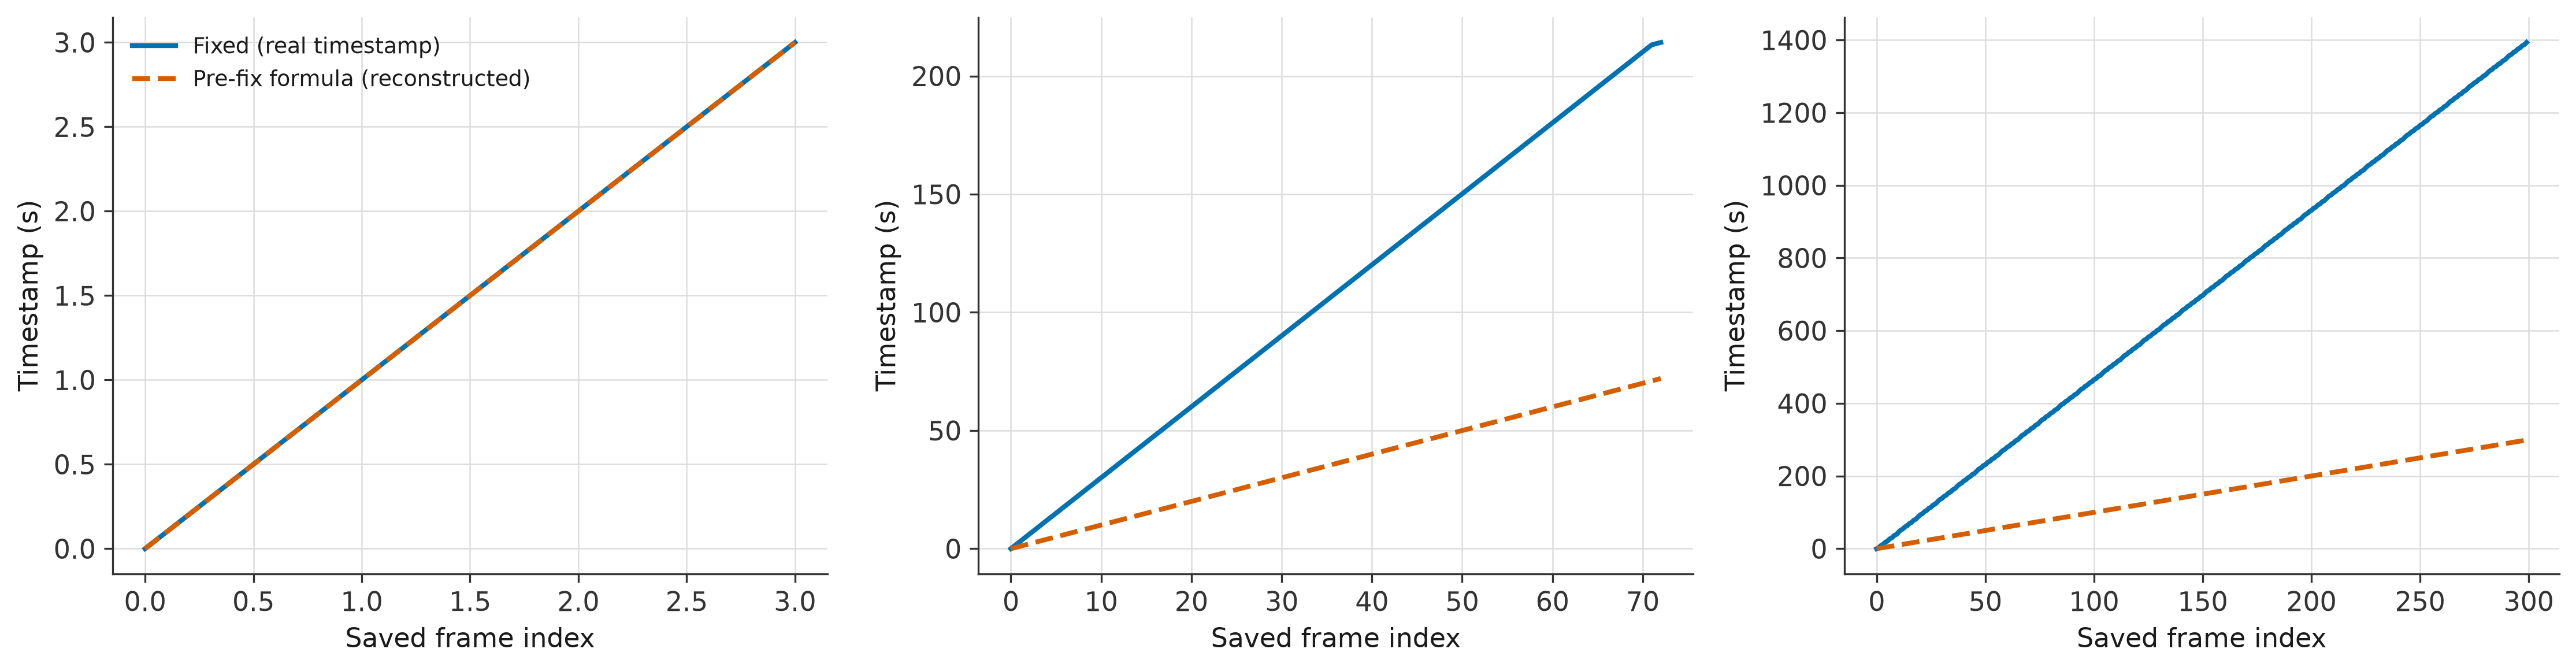
\includegraphics[width=\linewidth]{figures/fig1_timestamp_fidelity}}
\caption{Real (fixed) vs.\ reconstructed pre-fix timestamps, by saved frame index, left to right: \texttt{session1} (3.0\,s, 4 frames), \texttt{obama} (214.2\,s, 73 frames), \texttt{clancy1} (1393.4\,s, 300 frames). Drift grows with video length as predicted.}
\label{fig:ts}
\end{figure}

\subsection{Multi-modal retrieval}

Forty documents were sampled per modality from the real indexes (697 speech segments,
81 captions, 228 OCR entries, pooled across all seven videos); each document's leading
words became a query, and retrieval was scored both strictly (recovering the exact
source frame) and content-aware (recovering any frame with matching stored text, since
captions and OCR text are frequently near-duplicated across nearby frames). Speech
retrieval was solid (MRR 0.47 exact / 0.57 content-aware); caption and OCR retrieval
were weak (MRR $\approx$ 0.02 each; Fig.~\ref{fig:retrieval}). This traces to a real,
identifiable cause rather than a metric artifact: only 29 of 81 stored captions were
unique text, and only 11 of 228 OCR entries were unique, indicating heavily templated
caption generation and highly repetitive OCR output that the retrieval embedding
struggles to re-discriminate.

\begin{figure}[t]
\centering
\begin{subfigure}[b]{0.32\linewidth}
\centering
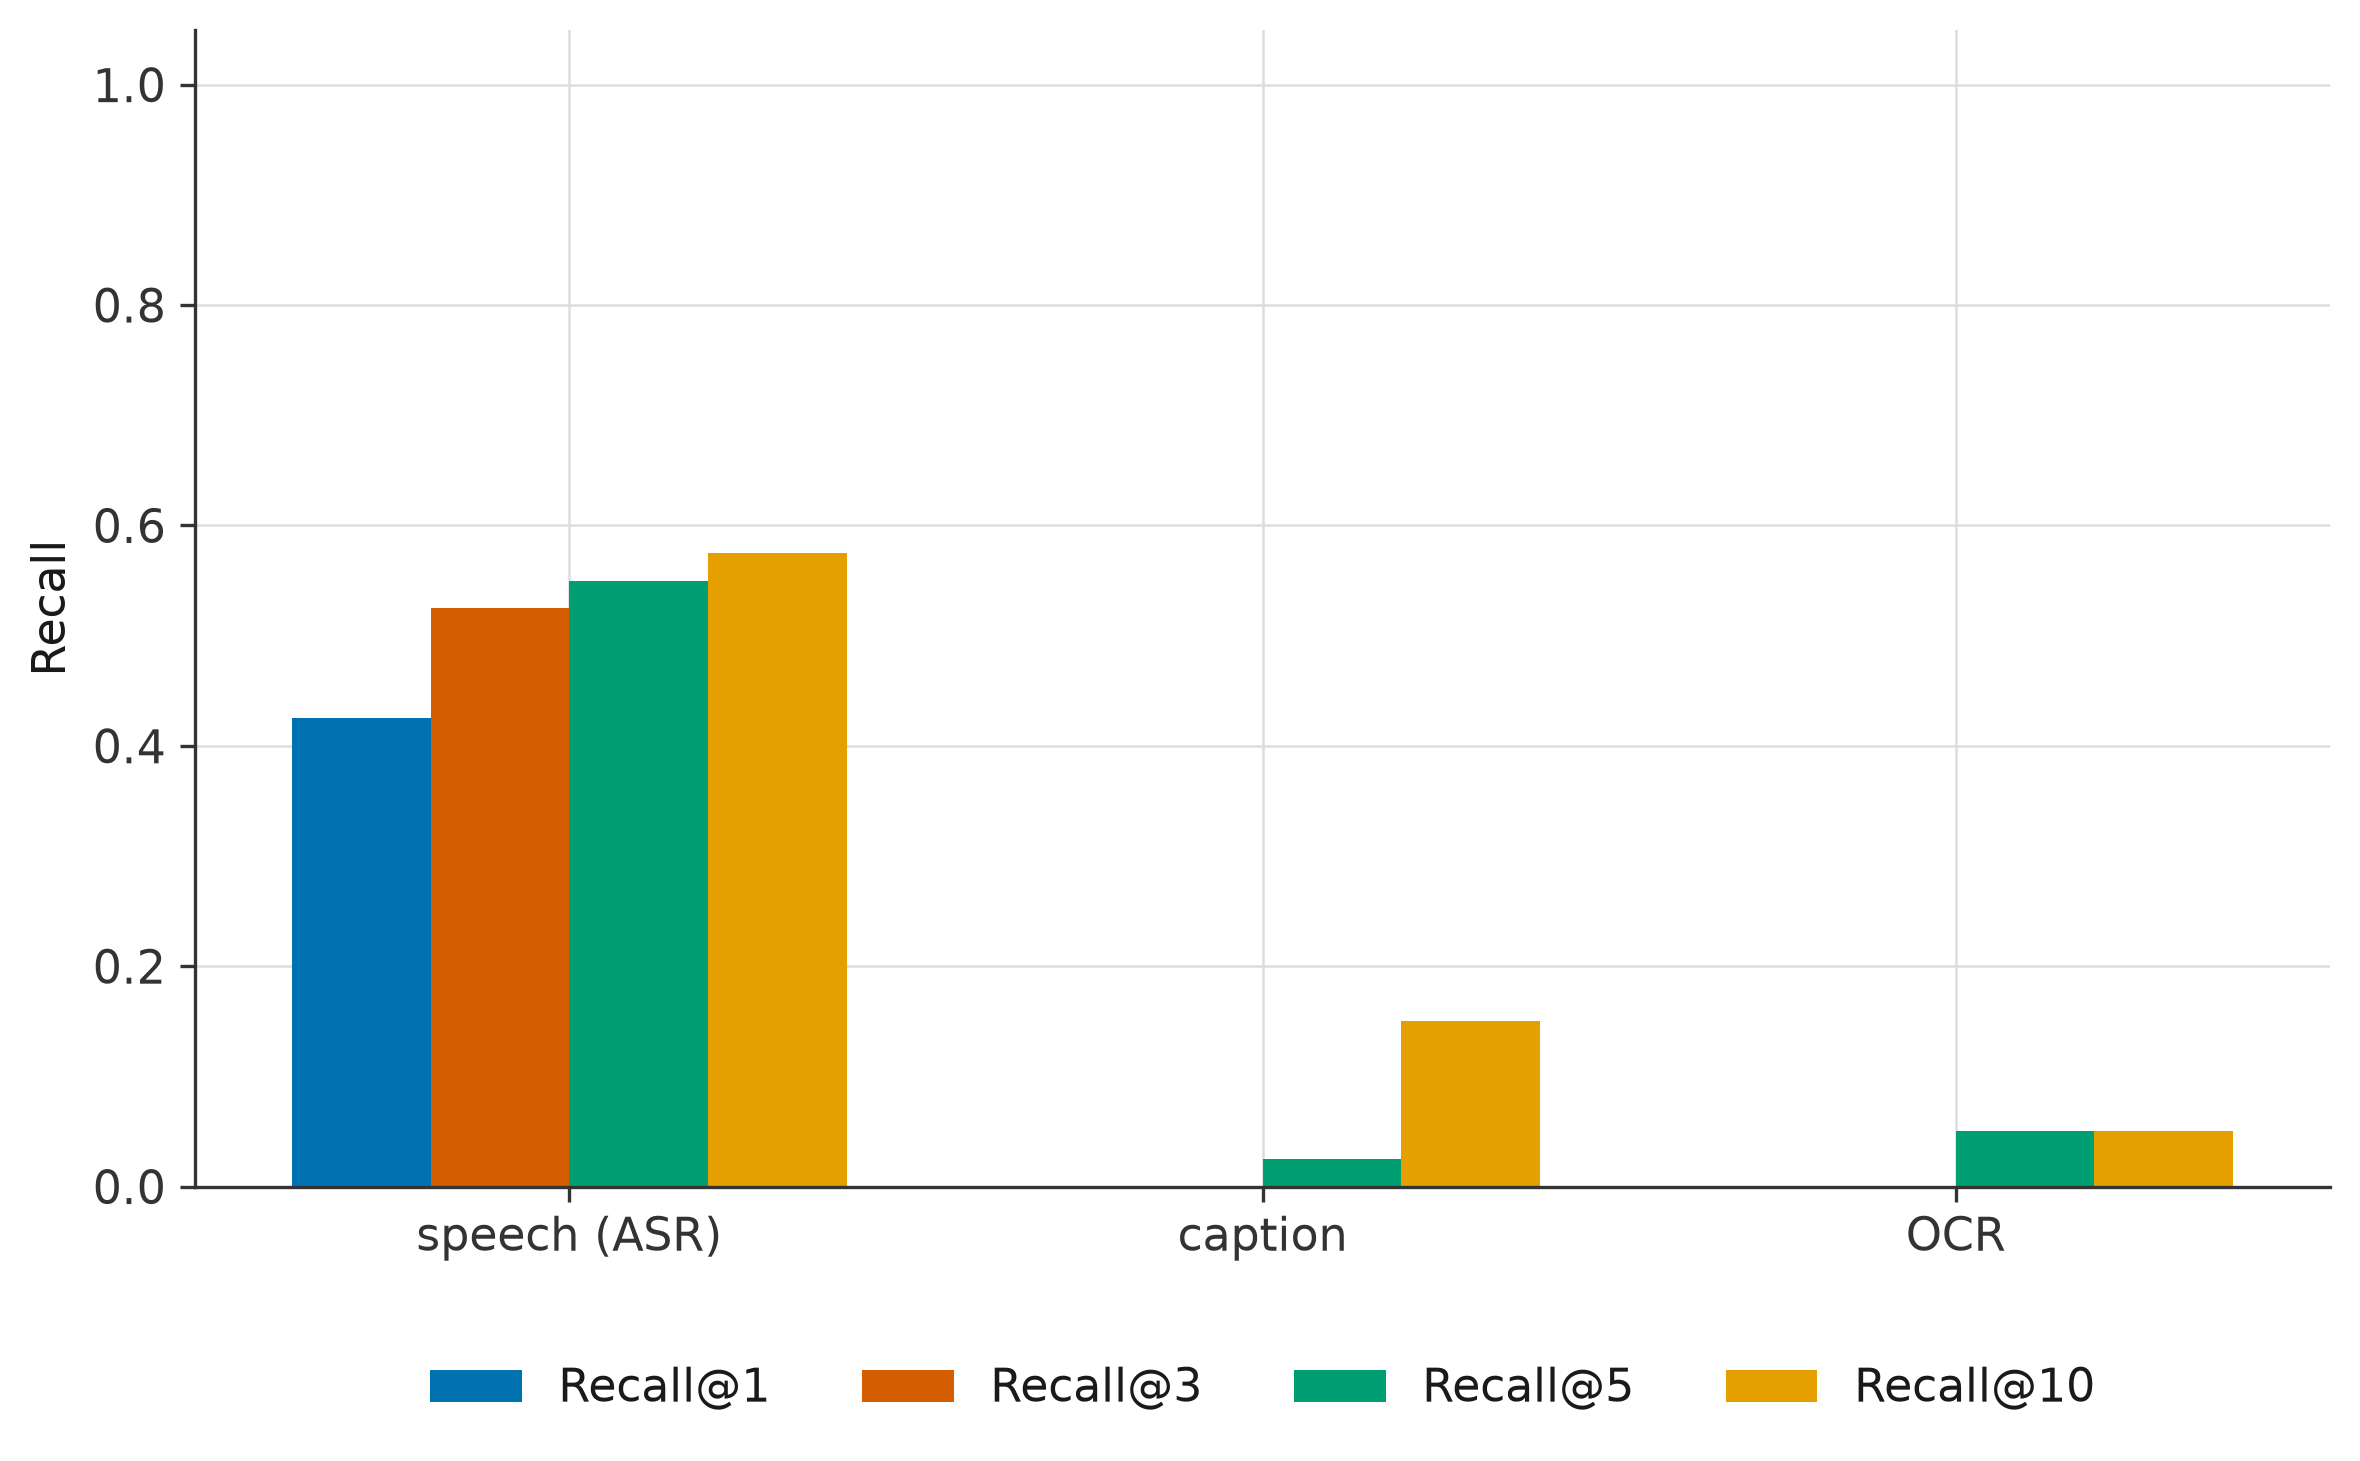
\includegraphics[width=\linewidth]{figures/fig2_retrieval_recall}
\caption{Recall@k by modality (exact-source-frame criterion).}
\label{fig:retrieval}
\end{subfigure}\hfill
\begin{subfigure}[b]{0.32\linewidth}
\centering
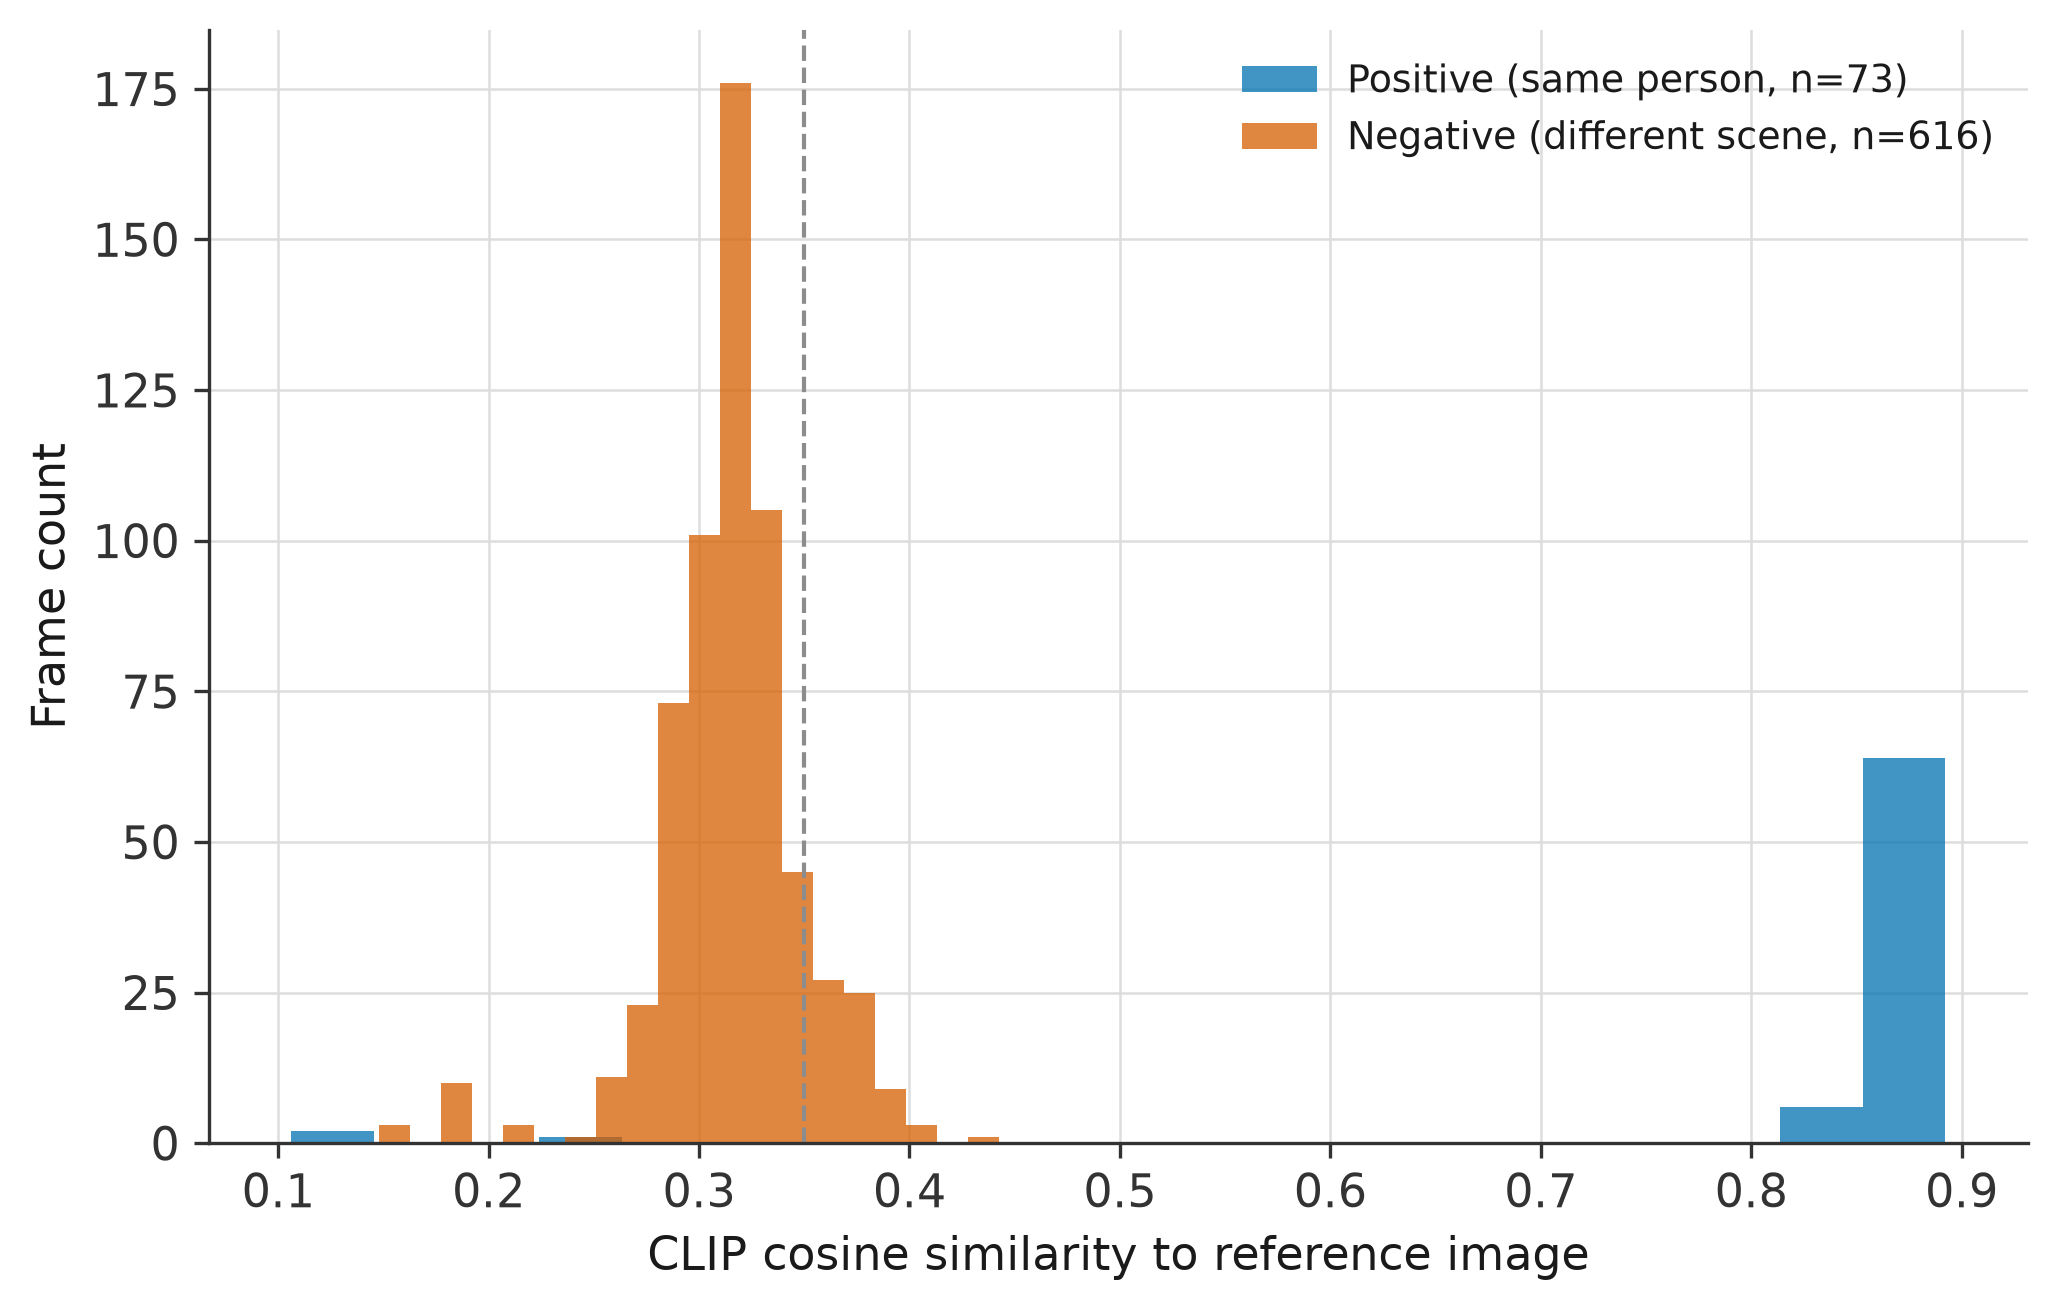
\includegraphics[width=\linewidth]{figures/fig3_image_search_scores}
\caption{CLIP similarity score distribution by class.}
\label{fig:imgsearch}
\end{subfigure}\hfill
\begin{subfigure}[b]{0.32\linewidth}
\centering
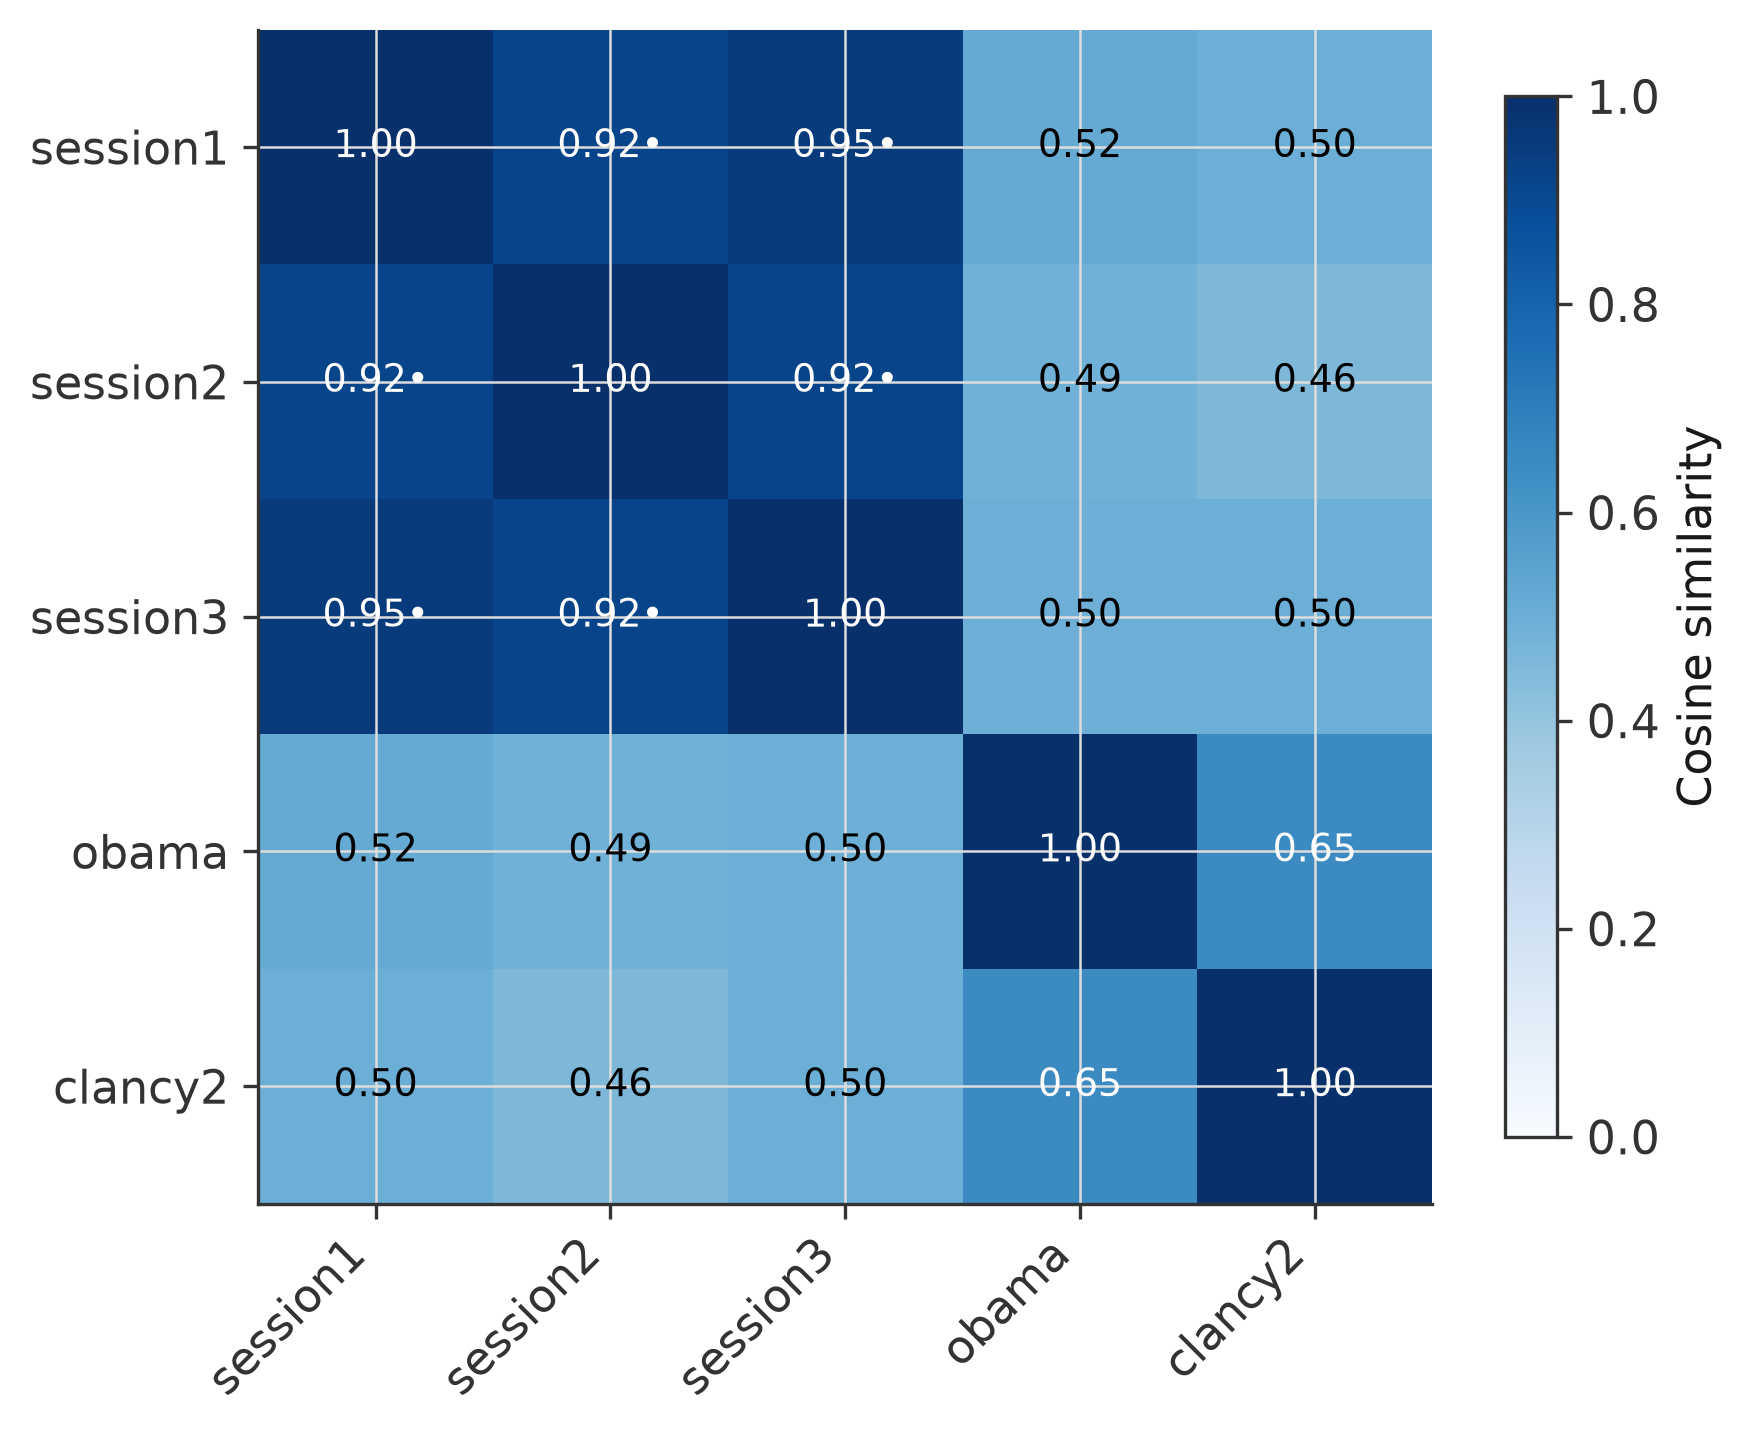
\includegraphics[width=\linewidth]{figures/fig4_speaker_similarity}
\caption{Pairwise voiceprint cosine similarity.}
\label{fig:speaker}
\end{subfigure}

\medskip
\begin{subfigure}[b]{0.32\linewidth}
\centering
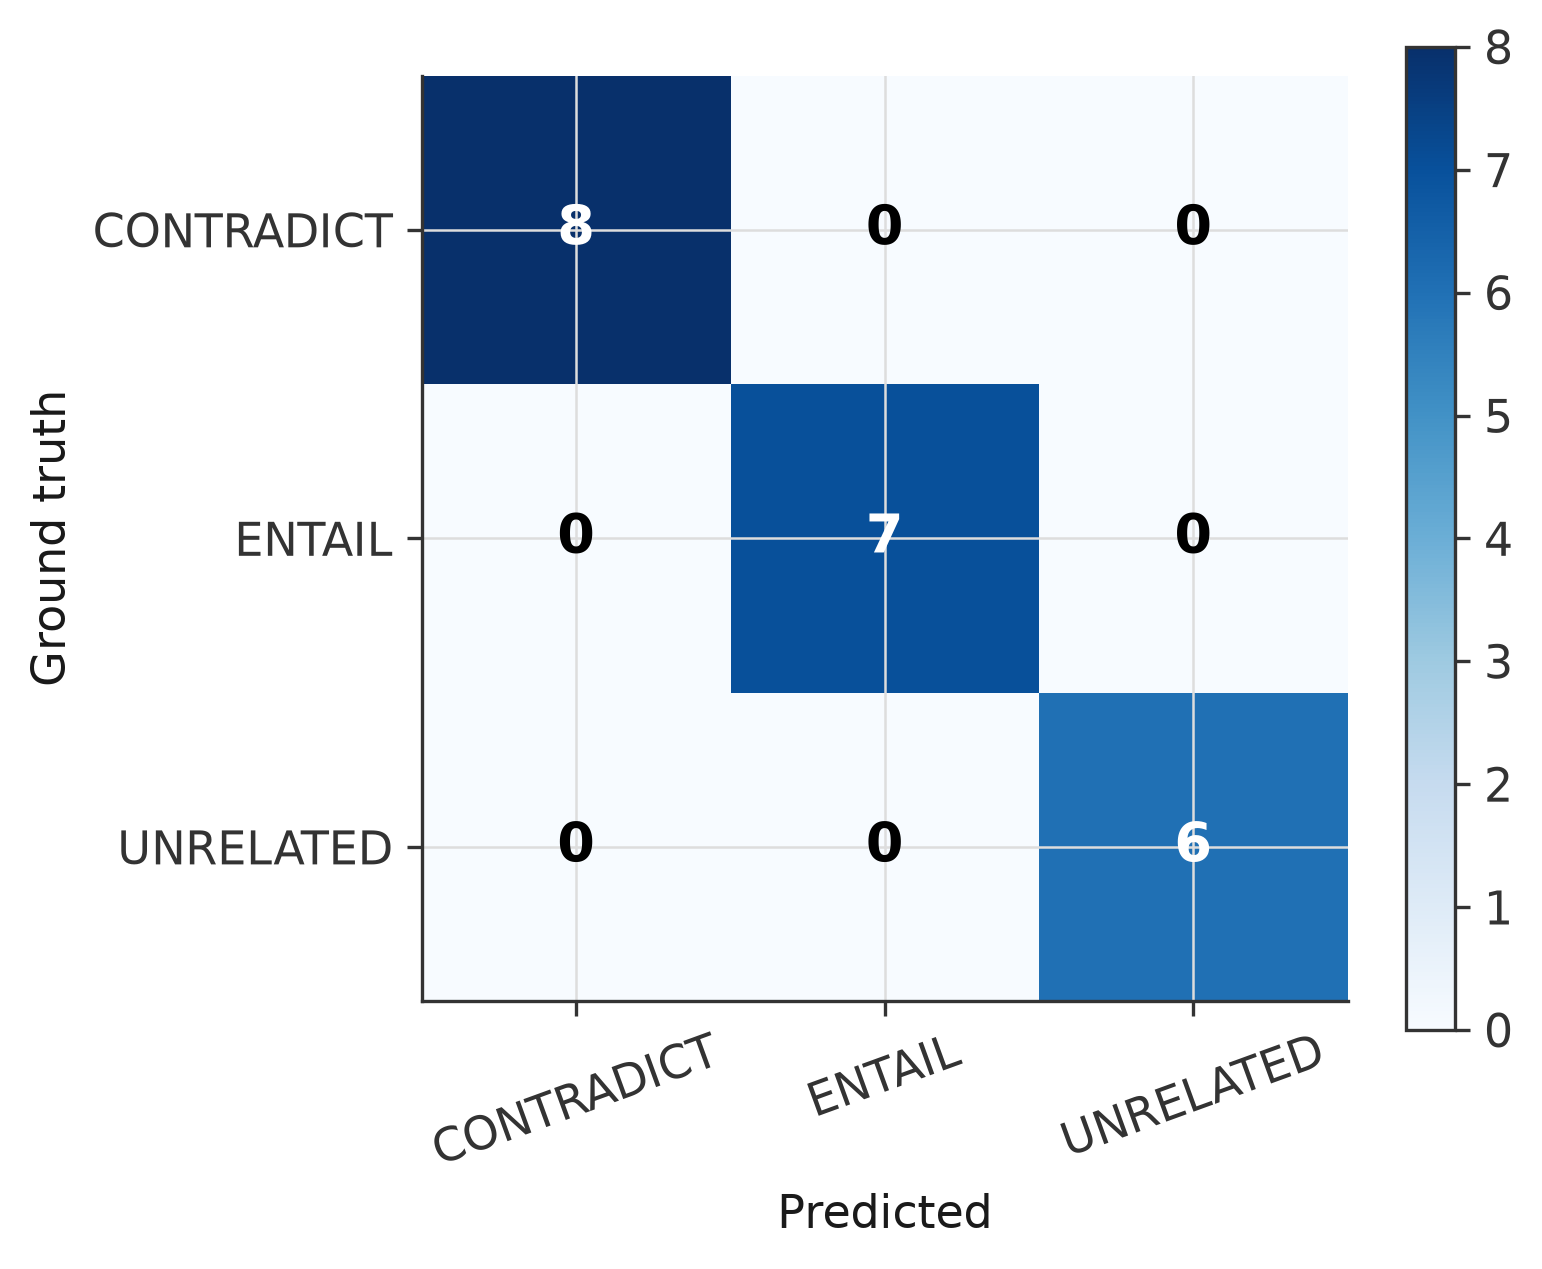
\includegraphics[width=\linewidth]{figures/fig5_contradiction_confusion}
\caption{Contradiction classifier confusion matrix.}
\label{fig:contra}
\end{subfigure}\hfill
\begin{subfigure}[b]{0.32\linewidth}
\centering
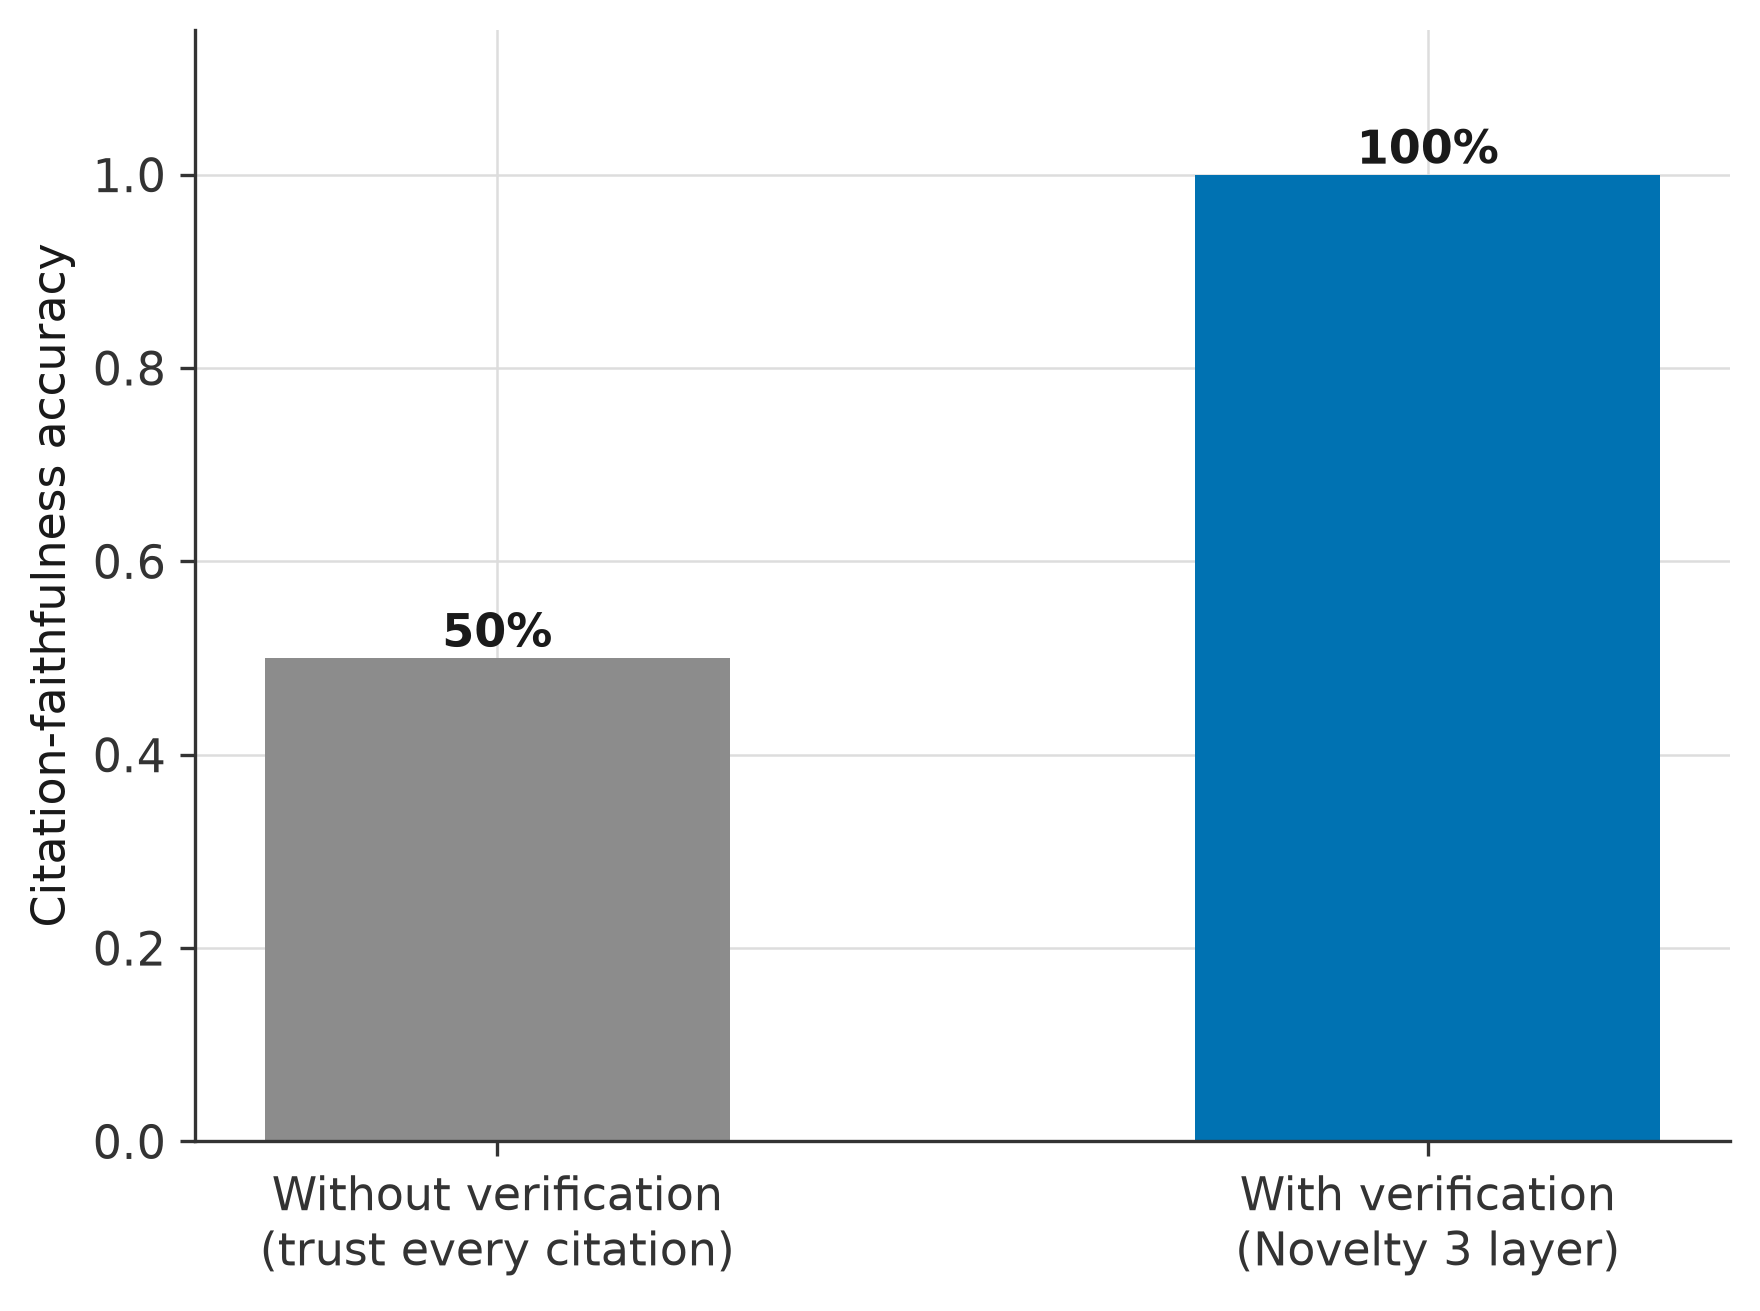
\includegraphics[width=\linewidth]{figures/fig6_citation_verification}
\caption{Citation faithfulness, with vs.\ without verification.}
\label{fig:citation}
\end{subfigure}\hfill
\begin{subfigure}[b]{0.32\linewidth}
\centering
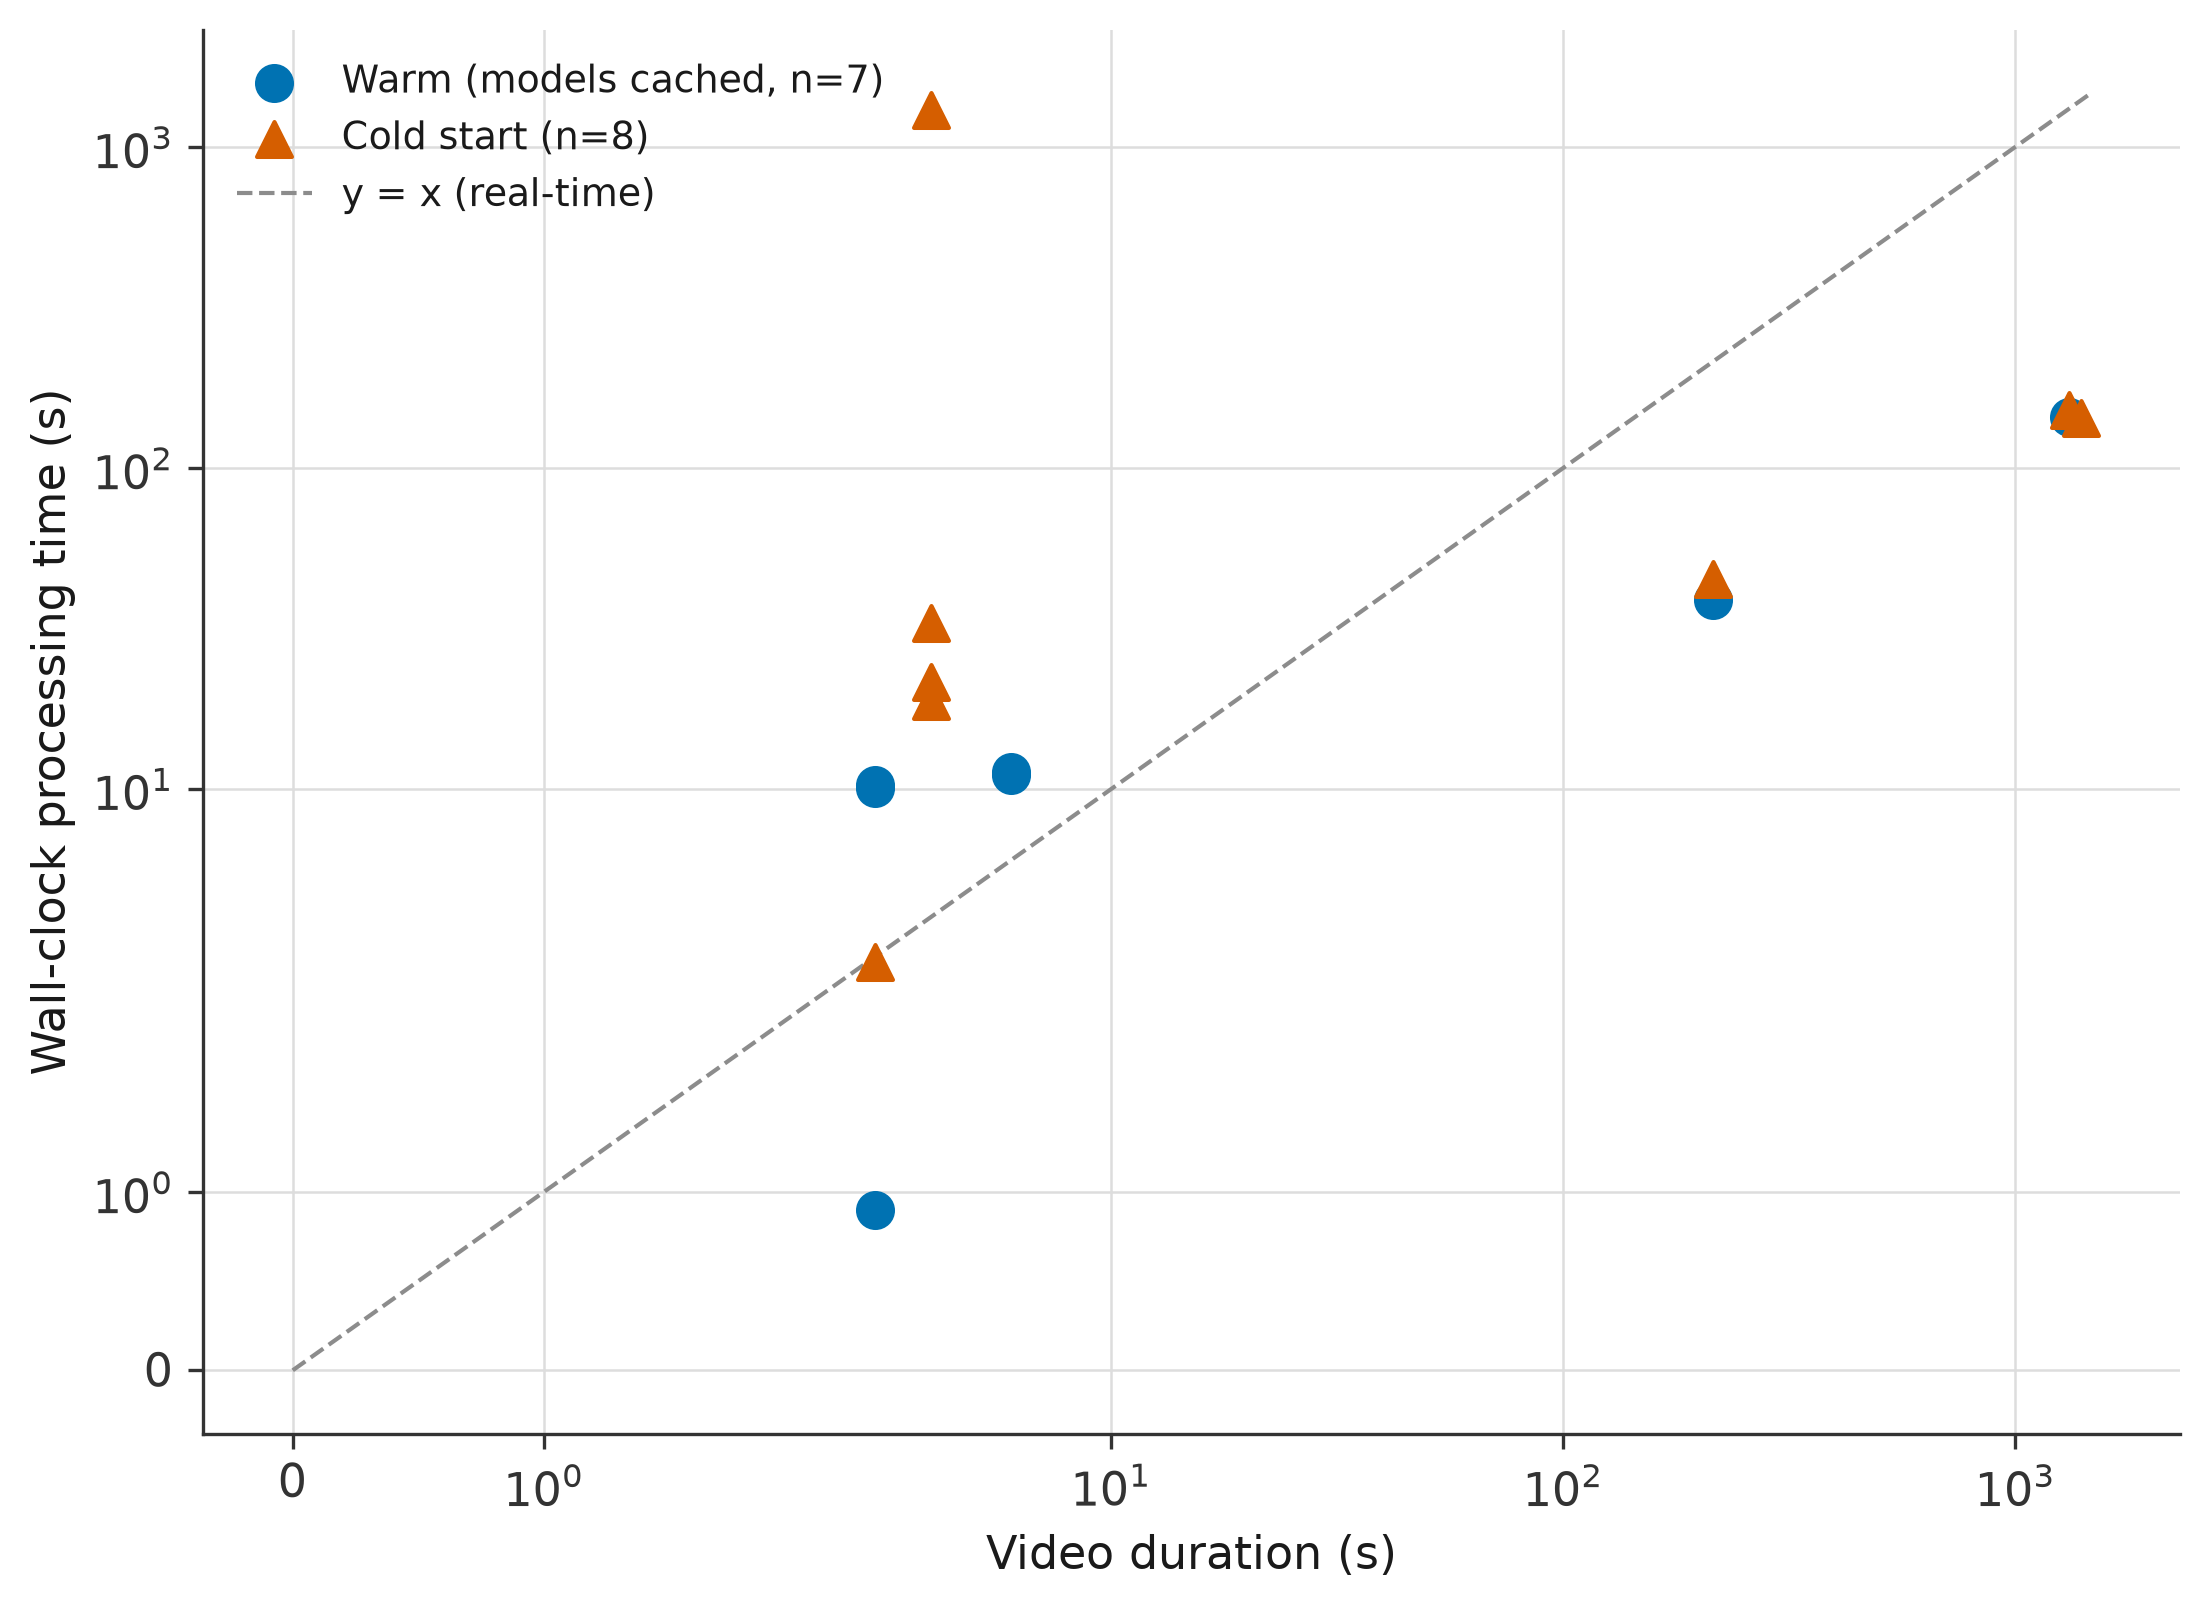
\includegraphics[width=\linewidth]{figures/fig7_scalability}
\caption{Processing time vs.\ video duration.}
\label{fig:scale}
\end{subfigure}
\caption{Evaluations 2--7 (Sections \ref{sec:results}): retrieval, image search, speaker
verification, contradiction detection, citation verification, and scalability. Full
discussion of each panel is in the corresponding subsection's text.}
\label{fig:grid}
\end{figure}

\subsection{Image-to-video person search}

A face crop taken from the \texttt{obama} video was scored against every stored frame
across all seven videos (73 true-positive frames, 616 true-negative frames from
unrelated scenes). The classifier itself separates the classes almost perfectly
(ROC-AUC 0.959, EER 0.021 at a similarity threshold of 0.842; Fig.~\ref{fig:imgsearch}
shows two essentially non-overlapping score clusters). However, at the thresholds
actually deployed in the running system (0.35 for general search, 0.30 as a hard
confidence gate), precision was far lower than the AUC alone suggests: 48.3\% and
13.1\% respectively, both at 95.9\% recall, because those thresholds sit inside the
negative-class distribution rather than in the empty gap between the two clusters
(approximately 0.45--0.80). Raising the deployed threshold into that gap would be
expected to move precision toward 1.0 at no recall cost on this test set.

\subsection{Cross-session speaker verification}

Every voiceprint the running system had captured (five: \texttt{session1/2/3}, one
Clancy-trial speaker, and \texttt{obama}) was compared pairwise. \texttt{session1/2/3}
share a synthesized voice (true positive pairs by construction); every other pair is a
genuinely different voice (true negative). At $n=10$ pairs (3 positive, 7 negative),
ROC-AUC was 1.0, and precision/recall at the deployed matching threshold (0.75) were
both 1.0 (Fig.~\ref{fig:speaker}). Same-speaker similarities clustered at 0.92--0.95;
different-speaker similarities at 0.46--0.65, a comfortable margin either side of the
threshold. This is a small-$n$ result for a specific, stated reason: one real
courtroom video's four diarized speakers were processed before the memory-overflow fix
(Section \ref{sec:impl}) and never obtained a captured voiceprint, so they could not be
included as additional negative pairs.

\subsection{Contradiction detection}

Eighteen statement pairs (six per class, authored for this evaluation with
deliberately unambiguous ground truth, independent of any real transcript) plus three
pairs produced end-to-end by the system's own synthetic cross-session test were run
through the production contradiction classifier. At $n=21$, accuracy was 100\% across
all three classes (Fig.~\ref{fig:contra}), and the false-positive rate on the
\texttt{CONTRADICT} class specifically was 0\%, a result worth isolating since in a
legal-evidence tool a false contradiction flag is a more costly failure mode than a
missed one. This is a clean-case sanity result, not a stress test of the genuinely
subtle, partially-worded contradictions real testimony produces; Section
\ref{sec:discussion} describes what a properly powered follow-up requires.

\subsection{Citation verification}

Ten claims, each paired with a real \texttt{(video, timestamp)} from the \texttt{obama}
video (five accurately summarizing what is discussed at that point, five deliberately
mismatched to an unrelated topic at the same timestamp), were scored by the production
verifier as a binary classifier. Verifier accuracy was 100\%, versus 50\% for the naive
``trust every citation'' baseline that represents the system with this layer removed
(Fig.~\ref{fig:citation}). The clean 50-point gap is this layer's directly
measurable contribution on this balanced test set.

\subsection{Scalability}

Real wall-clock timestamps from every video processed during development ($n=15$) were
paired with video duration and split into cold-start runs (first upload after a server
restart, paying a one-time model-loading cost) and warm runs (Fig.~\ref{fig:scale}).
Excluding one extreme outlier (the very first upload of the project, which paid a
network model-\emph{download} cost rather than an ordinary disk-cache reload), ordinary
cold starts cost a mean 59.3\,s of loading overhead. Warm-state processing of the two
real $\sim$22-minute courtroom recordings completed in 143--151\,s, roughly $9\times$
faster than real time, since frame extraction is bounded by a compute budget rather
than growing linearly with duration. Reprocessing the same 1316\,s video before and
after the voiceprint memory-overflow fix (Section \ref{sec:impl}) cost 144\,s and
151\,s respectively, a $\sim$5\% difference, confirming that fix's value is
correctness (the pre-fix run silently produced no usable voiceprint for that speaker),
not speed.

\section{Discussion and Limitations}
\label{sec:discussion}

Several results above are reported at exploratory scale by necessity rather than
choice, and we state plainly what a stronger version of each would require. Speaker
verification (Section \ref{sec:novelty1}) needs a multi-session archive in which the
\emph{same} speakers genuinely recur across separately recorded sessions; the two real
courtroom recordings used here happen to feature different witnesses, which is useful
as a negative-pair test but cannot establish a true-positive cross-session matching
rate at scale. Contradiction detection (Section \ref{sec:novelty2}) was validated on
deliberately unambiguous pairs; a rigorous benchmark needs real or realistically
paraphrased courtroom statement pairs labeled by at least two independent human
annotators, with inter-annotator agreement (Cohen's $\kappa$) reported alongside model
accuracy, since contradiction judgments on real testimony are frequently genuinely
subjective. Citation verification (Section \ref{sec:novelty3}) was scored as a binary
classifier on designed cases; the system's real-world hallucination rate requires
sampling unprompted generated answers and having a human judge each citation.

The retrieval evaluation (Section \ref{sec:results}, caption/OCR) points at two
concrete, independent engineering questions rather than a single vague weakness: does
the current captioning approach produce sufficiently diverse per-frame descriptions, and
is a general-purpose vision-language text encoder the right embedding choice for
literal short-string OCR matching, or would a dedicated text embedder perform better on
that specific sub-index. The image-search evaluation (Section \ref{sec:results}) yields
an immediately actionable recommendation: raise the deployed similarity threshold,
precisely because the classifier's own separation between classes is already strong. The
problem is calibration, not discriminative power.

Finally, no evaluation in this paper measures end-to-end answer quality as a human
user of the system would judge it, nor compares the full architecture against a
simpler baseline (e.g., keyword search over the raw transcript with no decouple, merge,
or verification layers). Both are necessary before any claim of the full pipeline's
value over a naive alternative can be made with confidence, and are the most important
items for future work.

\section{Conclusion and Future Work}
\label{sec:conclusion}

We presented a multimodal RAG system for courtroom video evidence with three layers
targeted specifically at legal use: human-confirmed cross-session speaker
identification, persistent testimony memory with LLM-based contradiction detection, and
independent citation verification with tamper-evident hashing. We evaluated all
layers, plus the underlying retrieval architecture, against a corpus that includes real
public-domain speech and real courtroom trial footage. Results were strong where the
classifiers themselves are concerned (ROC-AUC $\geq$ 0.959 for both image search and
speaker verification; 100\% accuracy on designed contradiction and citation-verification
test sets) and honestly weak in two places we identified and explained rather than
omitted: caption/OCR retrieval, and image-search threshold calibration under real-world
class imbalance. Future work centers on closing the scale gaps named in Section
\ref{sec:discussion}: a multi-session real trial archive for a properly powered speaker
re-identification benchmark, human-annotated contradiction pairs with inter-annotator
agreement, a sampled real-answer citation audit, an OCR-embedding ablation, Diarization
Error Rate evaluated in line with standard practice \cite{ryant2020dihard} against a
manually labeled reference, and an end-to-end human evaluation of answer quality against
a non-trivial baseline system.

\section*{Acknowledgements}

[Acknowledgements to be added.]

\appendix
\section{Evaluation artifacts}
\label{app:artifacts}
All evaluation scripts, raw metric outputs, and figures reported in Section
\ref{sec:results} are available alongside the system implementation for independent
reproduction; each script re-derives its metrics directly from the running system's
own indexes and stores rather than from cached or hand-entered numbers.

\begin{thebibliography}{}

\bibitem{lewis2020}
Lewis, P., Perez, E., Piktus, A., Petroni, F., Karpukhin, V., Goyal, N., K\"{u}ttler, H., Lewis, M., Yih, W., Rockt\"{a}schel, T., Riedel, S., Kiela, D. (2020) ``Retrieval-Augmented Generation for Knowledge-Intensive NLP Tasks.'' {\it Advances in Neural Information Processing Systems (NeurIPS)} {\bf 33}: 9459--9474.

\bibitem{radford2021}
Radford, A., Kim, J.W., Hallacy, C., Ramesh, A., Goh, G., Agarwal, S., Sastry, G., Askell, A., Mishkin, P., Clark, J., Krueger, G., Sutskever, I. (2021) ``Learning Transferable Visual Models From Natural Language Supervision.'' {\it Proceedings of the 38th International Conference on Machine Learning (ICML)}: 8748--8763.

\bibitem{radford2023}
Radford, A., Kim, J.W., Xu, T., Brockman, G., McLeavey, C., Sutskever, I. (2023) ``Robust Speech Recognition via Large-Scale Weak Supervision.'' {\it Proceedings of the 40th International Conference on Machine Learning (ICML)}: 28492--28518.

\bibitem{li2022}
Li, J., Li, D., Xiong, C., Hoi, S. (2022) ``BLIP: Bootstrapping Language-Image Pre-training for Unified Vision-Language Understanding and Generation.'' {\it Proceedings of the 39th International Conference on Machine Learning (ICML)}: 12888--12900.

\bibitem{bredin2020}
Bredin, H., Yin, R., Coria, J.M., Gelly, G., Korshunov, P., Lavechin, M., Fustes, D., Titeux, H., Bouaziz, W., Gill, M. (2020) ``pyannote.audio: neural building blocks for speaker diarization.'' {\it IEEE International Conference on Acoustics, Speech and Signal Processing (ICASSP)}: 7124--7128.

\bibitem{wan2018}
Wan, L., Wang, Q., Papir, A., Moreno, I.L. (2018) ``Generalized End-to-End Loss for Speaker Verification.'' {\it IEEE International Conference on Acoustics, Speech and Signal Processing (ICASSP)}: 4879--4883.

\bibitem{jocher2023}
Jocher, G., Chaurasia, A., Qiu, J. (2023) ``YOLO by Ultralytics.'' \url{https://github.com/ultralytics/ultralytics}.

\bibitem{vaswani2017}
Vaswani, A., Shazeer, N., Parmar, N., Uszkoreit, J., Jones, L., Gomez, A.N., Kaiser, {\L}., Polosukhin, I. (2017) ``Attention Is All You Need.'' {\it Advances in Neural Information Processing Systems (NeurIPS)} {\bf 30}: 5998--6008.

\bibitem{yin2023survey}
Yin, S., Fu, C., Zhao, S., Li, K., Sun, X., Xu, T., Chen, E. (2023) ``A Survey on Multimodal Large Language Models.'' {\it arXiv preprint} arXiv:2306.13549.

\bibitem{ryant2020dihard}
Ryant, N., Church, K., Cieri, C., Du, J., Ganapathy, S., Liberman, M. (2020) ``Third DIHARD Challenge Evaluation Plan.'' {\it arXiv preprint} arXiv:2006.05815.

\bibitem{redmon2016}
Redmon, J., Divvala, S., Girshick, R., Farhadi, A. (2016) ``You Only Look Once: Unified, Real-Time Object Detection.'' {\it IEEE Conference on Computer Vision and Pattern Recognition (CVPR)}: 779--788.

\bibitem{malkov2020hnsw}
Malkov, Y.A., Yashunin, D.A. (2020) ``Efficient and Robust Approximate Nearest Neighbor Search Using Hierarchical Navigable Small World Graphs.'' {\it IEEE Transactions on Pattern Analysis and Machine Intelligence} {\bf 42} (4): 824--836.

\bibitem{williams2018multinli}
Williams, A., Nangia, N., Bowman, S.R. (2018) ``A Broad-Coverage Challenge Corpus for Sentence Understanding through Inference.'' {\it Proceedings of the 2018 Conference of the North American Chapter of the Association for Computational Linguistics: Human Language Technologies (NAACL-HLT)}: 1112--1122.

\bibitem{nie2020anli}
Nie, Y., Williams, A., Dinan, E., Bansal, M., Weston, J., Kiela, D. (2020) ``Adversarial NLI: A New Benchmark for Natural Language Understanding.'' {\it Proceedings of the 58th Annual Meeting of the Association for Computational Linguistics (ACL)}: 4885--4901.

\bibitem{min2023factscore}
Min, S., Krishna, K., Lyu, X., Lewis, M., Yih, W., Koh, P.W., Iyyer, M., Zettlemoyer, L., Hajishirzi, H. (2023) ``FActScore: Fine-grained Atomic Evaluation of Factual Precision in Long Form Text Generation.'' {\it Proceedings of the 2023 Conference on Empirical Methods in Natural Language Processing (EMNLP)}: 12076--12100.

\bibitem{manakul2023selfcheckgpt}
Manakul, P., Liusie, A., Gales, M.J.F. (2023) ``SelfCheckGPT: Zero-Resource Black-Box Hallucination Detection for Generative Large Language Models.'' {\it Proceedings of the 2023 Conference on Empirical Methods in Natural Language Processing (EMNLP)}: 9004--9017.

\bibitem{es2024ragas}
Es, S., James, J., Espinosa-Anke, L., Schockaert, S. (2024) ``RAGAs: Automated Evaluation of Retrieval Augmented Generation.'' {\it Proceedings of the 18th Conference of the European Chapter of the Association for Computational Linguistics: System Demonstrations (EACL)}: 150--158.

\bibitem{chalkidis2019legal}
Chalkidis, I., Androutsopoulos, I., Aletras, N. (2019) ``Neural Legal Judgment Prediction in English.'' {\it Proceedings of the 57th Annual Meeting of the Association for Computational Linguistics (ACL)}: 4317--4323.

\bibitem{ariai2024legalsurvey}
Ariai, F., Mackenzie, J., Demartini, G. (2024) ``Natural Language Processing for the Legal Domain: A Survey of Tasks, Datasets, Models, and Challenges.'' {\it arXiv preprint} arXiv:2410.21306.

\bibitem{touvron2024llama3}
Grattafiori, A., Dubey, A., Jauhri, A., et al. (2024) ``The Llama 3 Herd of Models.'' {\it arXiv preprint} arXiv:2407.21783.

\end{thebibliography}

\end{document}
